% !TeX root = document.tex
% !TeX encoding = UTF-8 Unicode

\chapter{Introdução}%
\label{chp:introducao}

Controle preditivo por modelo (\ac{MPC} --- \textit{Model Predictive Control}) é
uma técnica de controle avançada que utiliza o modelo do sistema para prever a
saída em momentos futuros e, com isso, gerar uma estratégia de controle. Esta
técnica pode ser aplicada em modelos contínuos, onde o tempo de amostragem é tão
pequeno que pode ser desconsiderado, ou discretos, onde o modelo já espera que
exista um certo tempo entre amostragens. A abordagem discreta será usada pois
melhor ilustra o funcionamento do \ac{MPC}, além de fornecer ao controlador mais
tempo para o processamento do próximo sinal de controle.

Em um modelo discreto o sinal é amostrado a cada \( \Delta{}t \) segundos. O
modelo não varia mais diretamente com o tempo, mas sim com o instante de
amostragem \( k \), que se associa com o tempo através do tempo de amostragem
como \( t = k\Delta{}t \). Assim, em um modelo discreto, ao se passar do tempo
\( 0 \) para o tempo \( \Delta{}t \) ou do tempo \( \Delta{}t \) para o tempo
\( 2\Delta{}t \), dizemos que se passou um instante.

Utilizando um modelo discreto pode-se então prever a saída do sistema para um
instante futuro, se as entradas que serão aplicadas ao sistema nos instantes
anteriores forem conhecidas. Pode-se então prever as saídas dos próximos \(N_p\)
instantes e utilizar técnicas de otimização para obtermos os próximos \(N_c\)
sinais de controle ótimos que levarão o sistema à referência. Ao utilizar apenas
o primeiro sinal de controle e recalcular os sinais de controle ótimos a todo
instante, o controlador será capaz de rejeitar ruídos e reagir a mudanças, como
a da referência. Esta técnica é chamada de Controle por Horizonte Recessivo e é
a base do \ac{MPC}~\cite{book:wang}.

A discretização foi feita no tempo, pois altera-se o modelo para que este não
mais dependa do tempo mas sim de um instante. Sistemas que dependem apenas do
tempo são chamados de sistemas a parâmetros concentrados (\ac{SPC}). No entanto
existem sistemas que não variam apenas no tempo, mas também no espaço, por
exemplo. Um exemplo é a transferência de calor em uma barra metálica, onde a
temperatura depende tanto do tempo quanto do ponto no espaço em que se faz a
medição. Sistemas que dependem de mais de uma variável são chamados de sistemas
a parâmetros distribuídos (\ac{SPD}). Sua modelagem é feita utilizando derivadas
parciais e equações diferenciais parciais (\ac{EDP})~\cite{masterthesis:nelson}.

Para ambos tipos de modelos é comum usar a modelagem por espaço de estados ao se
trabalhar com \ac{MPC}. Isso permite controlar facilmente sistemas com múltiplas
entradas e múltiplas saídas. No entanto, ao se trabalhar com espaço de estados,
é necessário que o valor de todos os estados sejam conhecidos, o que nem sempre
é possível, seja por limitações do sistema ou até mesmo físicas. Para resolver
este problema utiliza-se observadores.

O observador é um sistema que estima os estados de um modelo baseado nas
entradas e saídas do mesmo. O observador de Kalman, também conhecido como filtro
de Kalman, é uma formulação que permite estimar o modelo de forma precisa mesmo
na presença de ruídos, seja na leitura da saída ou dos próprios
estados~\cite{book:wang}.

\section{Definição do Problema}%
\label{sec:definicao-do-problema}

A Figura~\ref{fig:sensors-SPD} mostra os sensores do forno presente no
Laboratório de Sinais e Sistemas. Nela podemos ver os sensores \(S_1\) a \(S_5\)
e o fluxo de ar quente \( q \). Imagine que queiramos controlar a temperatura na
posição onde encontra-se o sensor \(S_3\), mas que apenas o sensor \(S_5\)
esteja funcionando. Com um modelo \ac{SPD} podemos ter dois modelos \ac{SPC}\@:
um que modele o fluxo de temperatura até o sensor \(S_3\) e um outro que modele
de \(S_3\) até \(S_5\), ambos interconectados. Desta forma podemos utilizar um
observador e a leitura do sensor \(S_5\) para estimar a temperatura no sensor
\(S_3\), e controlá-la mesmo sem fazer sua medição direta.

\begin{figure}[ht!]
    \centering
    \captionsetup{justification=centering}
    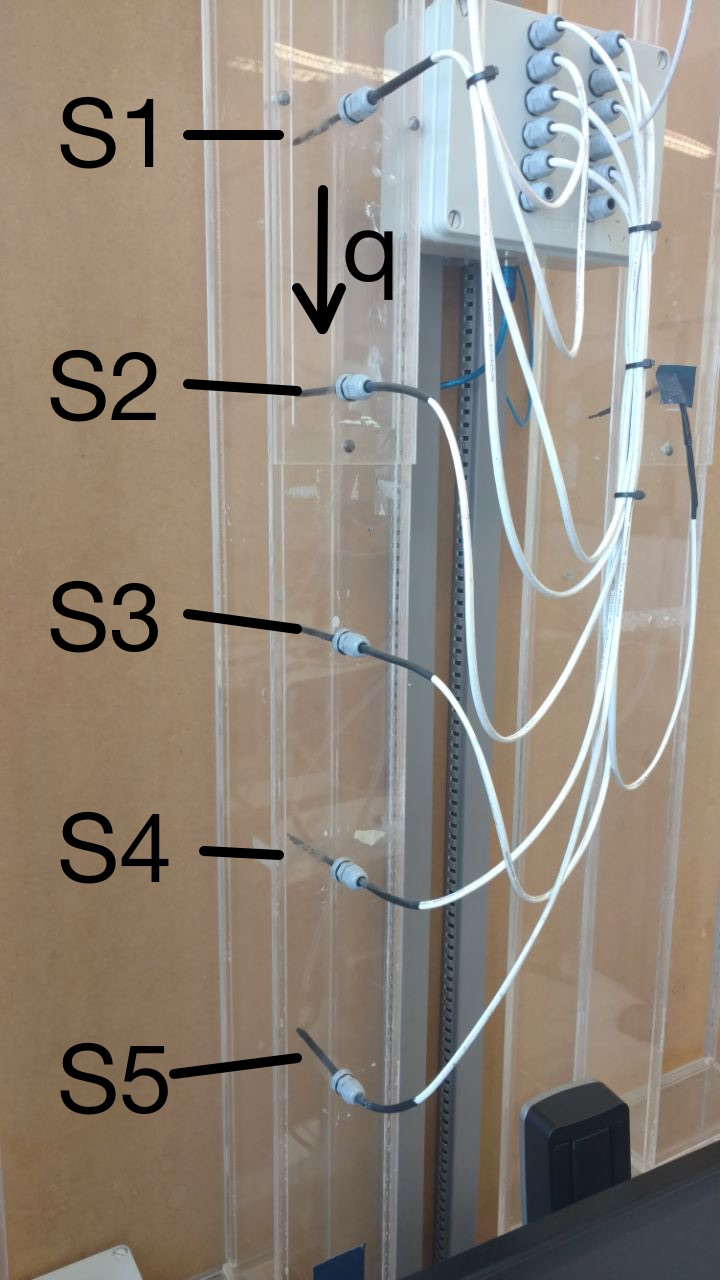
\includegraphics[height=0.5\linewidth]{imgs/planta-spd}
    \caption{Sensores da planta}%
    \label{fig:sensors-SPD}
\end{figure}

Propõe-se o desenvolvimento de controladores \ac{MPC} que utilizem os modelos
\ac{SPD} gerados pelo~\textcite{masterthesis:nelson} para controlar o processo
do forno conforme descrito acima. Além disso, os mesmos devem ser implementados
de forma a serem executados na plataforma desenvolvida pelo autor em sua
iniciação científica, utilizando esta oportunidade para corrigir problemas
encontrados e dar continuidade ao desenvolvimento da mesma.

\section{Objetivos}%
\label{sec:objectives}

Desenvolver um controlador do tipo \ac{MPC} com restrições com modelo \ac{SPD}
utilizando observadores do tipo Kalman e implementá-lo utilizando e adaptando a
plataforma de controle desenvolvida pelo proponente para uso no forno do
laboratório de sinais e sistemas. O objetivo pode ser assim dividido:

\begin{itemize}
      \item modificar a eletrônica da planta: instalar circuitos
            microprocessados com o intuito de controlar o acionamento do forno,
            fornecendo um caminho alternativo ao acionamento que já está
            implementado e permitindo a integração com a plataforma de controle;
      \item modificar a plataforma de controle: desenvolver driver específico
            para o forno, de forma a tornar o acionamento dos atuadores e a
            leitura dos sensores mais simples e direto para os futuros usuários;
      \item desenvolver o controlador \ac{MPC}\@: utilizar o modelo \ac{SPD}
            desenvolvido pelo~\textcite{masterthesis:nelson} para desenvolver um
            controlador \ac{MPC} com restrições na entrada e saída de forma a
            controlar a temperatura em um ponto diferente daquele onde está
            fisicamente instalado o sensor;
      \item implementar o controlador: utilizar a linguagem Python e a
            plataforma de controle para implementar o controlador e executar o
            controle da planta;
      \item comparar o desempenho do controlador: usar índices de desempenho
            para comparar o desempenho do controlador \ac{MPC} com controladores
            PI ou PID a serem desenvolvidos utilizando as técnicas
            de~\textcite{article:clarke} e~\textcite{article:martins};
      \item realizar melhorias na plataforma: ao utilizar a plataforma como
            usuário, espera-se encontrar dificuldades, erros e novas ideias que
            serão ser corrigidos/implementadas, como, por exemplo, recuperação
            de mensagens de erro salvas no banco de dados e exibição para o
            usuário e verificação de sintaxe de código digitado pelo usuário.
\end{itemize}

\section{Motivação}%
\label{sec:motivacao}

A principal motivação para o trabalho é poder fazer o controle de um processo
sem medir diretamente a variável controlada. Isto é interessante pois nem sempre
é possível medir diretamente a grandeza que se deseja controlar, seja por
restrições físicas (como colocar um sensor no centro de um alto-forno?) ou por
questões financeiras.

A escolha do controlador \ac{MPC} se tornou interessante por ser uma técnica
avançada de controle que ainda não é estudada no \textit{campus V}. Assim, além
da possibilidade de estudar uma técnica avançada, este trabalho contribui por
ser o primeiro trabalho a utilizar tal controlador no Grupo de Modelagem e
Controle de Sistemas Mecatrônicos.

\section{Estado da arte}%
\label{sec:estado-da-arte}

O uso de controladores \ac{MPC} com modelos \ac{SPD} não é novo. Sua maior
aplicação, no entanto, continua sendo na área da química, fabricação de aço e,
principalmente na indústria petroquímica. Ele foi desenvolvido inicialmente para
controle de processos químicos, onde o equipamento é caro, o processo é lento e
contém várias entradas, saídas e estados que devem ser restringidas em amplitude
e taxa de variação~\cite{article:cairano}.

Este cenário está mudando e outras indústrias --- com modelos com poucas
entradas e saídas, custo mais baixo e dinâmica mais rápida --- estão adotodando
os controladores \ac{MPC}\@. No entanto, isso apresenta alguns desafios no
desenvolvimento de controladores, pois o \textit{framework} \ac{MPC} não foi
desenvolvido para tais sistemas e possui limitações como, por exemplo, o alto
custo computacional. Trabalhos já estão sendo desenvolvidos para minimizar ou
sanir tais problemas~\cite{article:cairano}.

Em ambientes industriais é comum o uso de computadores lógicos programáveis para
fazer a interface com o hardware. No meio acadêmico, no entanto, utiliza-se
softwares como o \textit{MATLAB} e \textit{LabVIEW} para a prototipagem rápida.
Isto requer que o pesquisador recrie a interface gráfica e controle a aquisição
de dados manualmente, o que consome tempo que poderia ser gasto com a pesquisa.

Assim, uma plataforma que faça a interface com o hardware e possibilite a
execução de um controlador de forma transparente permite que o pesquisador se
concentre nestes estudos e não se preocupe com detalhes da implementação da
aquisição dos dados. Tal ferramenta também permitiria ao pesquisador
interagir com CLPs, desenvolvendo e testando controladores de forma fácil em
uma linguagem simples (Python) sem se preocupar com todas as nuâncias das
linguagens LADDER utilizadas nos CLPs, podendo implementar seu controlador nesta
linguagem limitada apenas ao final, quando este tiver sido devidamente testado e
otimizado.

A aplicação de uma plataforma para controle em todos as plantas do laboratório
permite que os usuários possam migrar de uma planta para outra sem dificuldades.
Também permite que controladores e observadores desenvolvidos sejam testados em
diferentes plantas com poucas modificações, já que as interfaces seriam as
mesmas em todas elas.
